\documentclass{beamer}
\usepackage[utf8]{inputenc}

\usetheme{Madrid}
\usecolortheme{default}
\usepackage{amsmath,amssymb,amsfonts,amsthm}
\usepackage{mathtools}
\usepackage{txfonts}
\usepackage{tkz-euclide}
\usepackage{listings}
\usepackage{adjustbox}
\usepackage{array}
\usepackage{gensymb}
\usepackage{tabularx}
\usepackage{gvv}
\usepackage{lmodern}
\usepackage{circuitikz}
\usepackage{tikz}
\lstset{literate={·}{{$\cdot$}}1 {λ}{{$\lambda$}}1 {→}{{$\to$}}1}
\usepackage{graphicx}

\setbeamertemplate{page number in head/foot}[totalframenumber]

\usepackage{tcolorbox}
\tcbuselibrary{minted,breakable,xparse,skins}



\definecolor{bg}{gray}{0.95}
\DeclareTCBListing{mintedbox}{O{}m!O{}}{%
  breakable=true,
  listing engine=minted,
  listing only,
  minted language=#2,
  minted style=default,
  minted options={%
    linenos,
    gobble=0,
    breaklines=true,
    breakafter=,,
    fontsize=\small,
    numbersep=8pt,
    #1},
  boxsep=0pt,
  left skip=0pt,
  right skip=0pt,
  left=25pt,
  right=0pt,
  top=3pt,
  bottom=3pt,
  arc=5pt,
  leftrule=0pt,
  rightrule=0pt,
  bottomrule=2pt,
  toprule=2pt,
  colback=bg,
  colframe=orange!70,
  enhanced,
  overlay={%
    \begin{tcbclipinterior}
    \fill[orange!20!white] (frame.south west) rectangle ([xshift=20pt]frame.north west);
    \end{tcbclipinterior}},
  #3,
}
\lstset{
    language=C,
    basicstyle=\ttfamily\small,
    keywordstyle=\color{blue},
    stringstyle=\color{orange},
    commentstyle=\color{green!60!black},
    numbers=left,
    numberstyle=\tiny\color{gray},
    breaklines=true,
    showstringspaces=false,
}

\title{5.2.16}
\date{September 13, 2025}
\author{Bhargav - EE25BTECH11013}

\begin{document}

\frame{\titlepage}
\begin{frame}{Question}
Solve the system of equations:
\begin{align}
3x - 5y &= 20 \\
6x - 10y &= 40
\end{align}
\end{frame}

\begin{frame}{Line Representation}
The equation of a line is
\begin{align}
\vec{n^T}\vec{x} = c
\end{align}

Line L:
\begin{align}
\myvec{3 & -5}\myvec{x \\ y}=20
\end{align}
Line K:
\begin{align}
\myvec{6 & -10}\myvec{x \\ y}=40
\end{align}
\end{frame}
\begin{frame}{Matrix Form}
These can be combined into matrix form:
\begin{align}
\myvec{3 & -5 \\ 6 & -10}\myvec{x \\ y} = \myvec{20 \\ 40}
\end{align}

The following augmented matrix can be solved by Gaussian elimination 
\begin{align}
\augvec{2}{1}{3 & -5 & 20 \\ 6 & -10 & 40} 
\xleftrightarrow{R_2 \leftarrow R_2 - 2R_1} 
\augvec{2}{1}{3 & -5 & 20 \\ 0 & 0 & 0}
\end{align}
\end{frame}

\begin{frame}{Rank and Reduced Equation}
We end up with only one non-zero row (Rank = 1):
\begin{align}
\myvec{3 & -5}\myvec{x \\ y} = 20
\end{align}

This represents a line in $\mathbb{R}^2$.
\end{frame}

\begin{frame}{General Solution}
The general solution is:
\begin{align}
\myvec{x \\ y} = \myvec{t \\ \frac{3t-20}{5}}, \quad t \in \mathbb{R}
\end{align}

\textbf{Conclusion:}  
The system has \textbf{infinitely many solutions}.
\end{frame}

\begin{frame}{Plot}
\begin{figure}[h!]
    \centering
    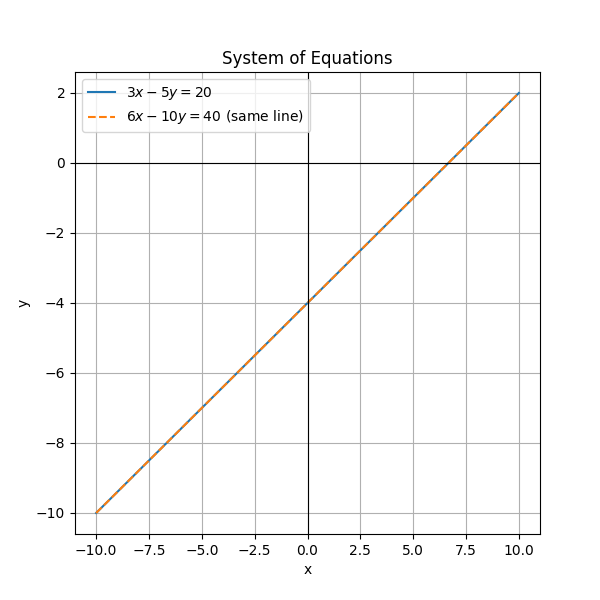
\includegraphics[height=0.5\textheight, keepaspectratio]{figs/Figure_1.png}
    \label{figure_1}
\end{figure}
\end{frame}

\begin{frame}[fragile]
    \frametitle{C Code}
    \begin{lstlisting}
#include <stdio.h>

// Function to compute y from first equation: y = (3x - 20)/5
double line1(double x) {
    return (3.0 * x - 20.0) / 5.0;
}

// Function to compute y from second equation: y = (6x - 40)/10
double line2(double x) {
    return (6.0 * x - 40.0) / 10.0;
}


    \end{lstlisting}
\end{frame}



\begin{frame}[fragile]
    \frametitle{Python + C Code}
    \begin{lstlisting}
import ctypes
import numpy as np
import matplotlib.pyplot as plt


lib = ctypes.CDLL("./liblines.so")

lib.line1.argtypes = [ctypes.c_double]
lib.line1.restype = ctypes.c_double

lib.line2.argtypes = [ctypes.c_double]
lib.line2.restype = ctypes.c_double


x_vals = np.linspace(-10, 10, 400)
y1 = np.array([lib.line1(float(x)) for x in x_vals])
y2 = np.array([lib.line2(float(x)) for x in x_vals])



    \end{lstlisting}
\end{frame}

\begin{frame}[fragile]
    \frametitle{Python + C Code}
    \begin{lstlisting}

plt.figure(figsize=(6,6))
plt.plot(x_vals, y1, label=r'$3x - 5y = 20$')
plt.plot(x_vals, y2, '--', label=r'$6x - 10y = 40$ (same line)')

plt.axhline(0, color='black', linewidth=0.8)
plt.axvline(0, color='black', linewidth=0.8)
plt.xlabel("x")
plt.ylabel("y")
plt.title("System of Equations (C + Python)")
plt.legend()
plt.grid(True)
plt.savefig("/Users/bhargavkrish/Desktop/BackupMatrix/ee25btech11013/matgeo/5.2.16/figs/Figure_1.png")
plt.show()



    \end{lstlisting}
\end{frame}

\begin{frame}[fragile]
    \frametitle{Python Code}
    \begin{lstlisting}

import numpy as np
import matplotlib.pyplot as plt

A = np.array([[3, -5],
              [6, -10]])
b = np.array([20, 40])
print("The system has no solution (inconsistent).")
x_vals = np.linspace(-10, 10, 400)
y1 = (3*x_vals - 20)/5
y2 = (6*x_vals - 40)/10
plt.figure(figsize=(6,6))
plt.plot(x_vals, y1, label=r'$3x - 5y = 20$')
plt.plot(x_vals, y2, '--', label=r'$6x - 10y = 40$ (same line)')


    \end{lstlisting}
\end{frame}

\begin{frame}[fragile]
    \frametitle{Python Code}
    \begin{lstlisting}

plt.axhline(0, color='black', linewidth=0.8)
plt.axvline(0, color='black', linewidth=0.8)
plt.xlabel("x")
plt.ylabel("y")
plt.title("System of Equations")
plt.legend()
plt.grid(True)
plt.savefig("/Users/bhargavkrish/Desktop/BackupMatrix/ee25btech11013/matgeo/5.2.16/figs/Figure_1.png")
plt.show()



    \end{lstlisting}
\end{frame}

\end{document}